\section{Validation}
In this section we will validate and prove that our implementation works as expected and we will look into the performance of the implementation compared to similar alternatives.
\subsection{Benchmark}
When you choose your protocol, performance is an important factor. It should be said that you would probably not want to choose AMQP for its blistering speed, but rather for its broadcast or its queuing abilities or its delivery guarantees. In high performance request-response scenarios peer-to-peer is what you want, but that is not possible with AMQP. Every message is routed through an exchange server. This has a performance strength in the scenario where you broadcast your message once and it is routed to many (thousands) of clients.

For benchmarking we have sought inspiration from the project Implementation of D-Bus support for Jolie\cite{D-Bus} as it has an excellent benchmarking suite for Jolie, but we have written our own tests.
\subsubsection{Test hardware}
For the benchmarking we used a quad core machine with 8 logical threads running Ubuntu Desktop 13.10 64-bit. We used RabbitMQ as the AMQP message queue server. RabbitMQ was installed on the same machine but in a virtual PC (VMWare).\\
The performance of AMQP should be slightly better with RabbitMQ running on a real server.\\
The performance in general should be quite a bit worse on a real network instead of a virtual one. Especially for AMQP as AMQP has more network calls.
\begin{itemize}
\item CPU: Intel i7 \#\# 2.3 GHz quad core
\item RAM: 8 GB DDR3
\item OS and swap disk: Samsung 840 Evo 1 TB
\item OS: Ubuntu Desktop 13.10 64-bit
\item Jolie version: 1.0 \#\#
\item Java Runtime Environment version: \#\#
\item RabbitMQ OS: Ubuntu Desktop 13.04 64-bit \#\#
\item RabbitMQ version: 3.3.0 \#\#
\item erlang version: R16B0 \#\#
\item VMWare Player version: \#\#
\item vCPUs: 2
\item Virtual RAM: 1 GB
\item Network: VMWare virtual network
\end{itemize}
\subsubsection{AMQP}
\noindent\begin{tikzpicture}[trim axis left]
  \begin{axis}[
    scale only axis,
    grid=major,
    scaled x ticks=false,
    scaled y ticks=false,
    ylabel=Time in seconds,
    ymin=0,
    ymax=300,
    ytick={0,50,...,300},
    xlabel=Subscribers,
    xmin=1,
    xmax=10,
    xtick=data,
    height=5cm,
    width=\textwidth,
    legend entries={Socket SOAP, AMQP SOAP},
    legend style={at={(0.05,0.95)},anchor=north west},
    axis lines=left
  ]
    \addplot+[smooth]table{onetomany_socket_soap.data};
    \addplot+[smooth]table{onetomany_amqp_soap.data};
  \end{axis}
\end{tikzpicture}


\noindent\begin{tikzpicture}[trim axis left]
  \begin{axis}[
    scale only axis,
    grid=major,
    scaled x ticks=false,
    scaled y ticks=false,
    ylabel=Time in seconds,
    ymin=0,
    ymax=25,
    ytick={0,5,...,25},
    xlabel=Subscribers,
    xmin=1,
    xmax=10,
    xtick=data,
    height=5cm,
    width=\textwidth,
    legend entries={Socket SODEP, AMQP SODEP, AMQP SVDEP},
    legend style={at={(0.05,0.95)},anchor=north west},
    axis lines=left
  ]
    \addplot+[smooth]table{onetomany_socket_sodep.data};
    \addplot+[smooth]table{onetomany_amqp_sodep.data};
    \addplot+[smooth]table{onetomany_amqp_svdep.data};
  \end{axis}
\end{tikzpicture}


\noindent\begin{tikzpicture}[trim axis left]
  \begin{axis}[
    scale only axis,
    grid=major,
    scaled x ticks=false,
    scaled y ticks=false,
    ylabel=Time in seconds,
    ymin=0,
    ymax=25,
    ytick={0,5,...,25},
    xlabel=Messages,
    xmin=1000,
    xmax=10000,
    xtick=data,
    height=5cm,
    width=\textwidth,
    legend entries={Socket SODEP, AMQP SODEP},
    legend style={at={(0.05,0.95)},anchor=north west},
    axis lines=left
  ]
    \addplot+[smooth]table{onetoone_socket_sodep.data};
    \addplot+[smooth]table{onetoone_amqp_sodep.data};
  \end{axis}
\end{tikzpicture}

\subsubsection{Socket}

\subsubsection{Conclusion}
AMQP performed quite a lot better than we expected. AMQP was easily out performed by socket which was not so surprising, but was surprisingly close in performance to \#\#

As expected AMQP had an huge advantage for broadcasting a message to many subscribers. \#\# was its strongest competitor because of its extremely low overhead and very direct communication. For small messages AMQP stood without competition at 1 message to \#\# subscribers and for large messages 1 to \#\# subscribers.
\subsection{The JoRBA Project}
\label{subsec:The JoRBA Project}
The JoRBA Project\cite{Jorba} (Jolie Rule-Based Adaptation framework) is a project about dynamic adaptation through the use of hooks and adaptation rules.

The project includes proof of concept software which is fairly large distributed system of communicating components. We downloaded the software and modified nothing but the location fields so it used our AMQP extension and our RabbitMQ message queue server as a relay for the communication between the components. We started seven components and they registered with the adaptation manager and the test client ran perfectly.

This was a great test of our request-response implementation.
\begin{figure}[H]
  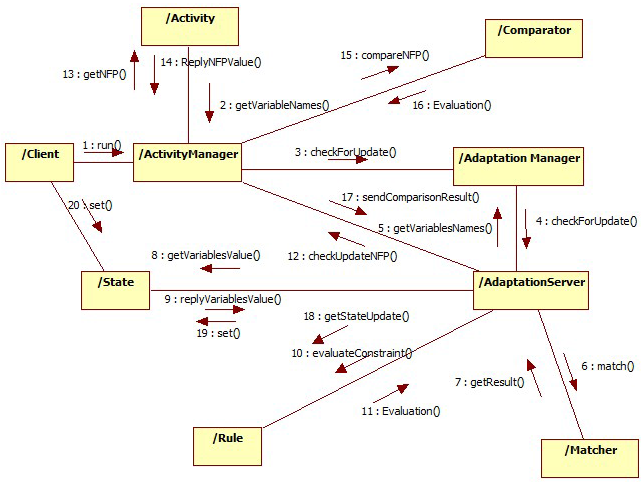
\includegraphics[width=\textwidth]{illustrations/Jorba.png}
  \caption{JoRBA collaboration diagram}
\end{figure}
\newpage
